\chapter{Event Reconstruction}
\label{chap:selection}

In order to target \ttDM production in the dilepton final state, where both top quarks have leptonically decaying W bosons, the selection criteria is compatible with that of SM \ttbar decays in the dilepton final state, but with an additional requirement that the event contain a moderate amount of \MET.

Sections ~\ref{subsec:leps} are dedicated to the necessary criteria each object in an event must adhere to for consideration as a potential signal event.

\section{Leptons}
\label{sec:leps}
A top and anti-top quark are expected in the signal event, and each emits a $\mathrm{W^+}$ and $\mathrm{W^-}$ respectively. The $\mathrm{W^\pm}$ boson in turn decays to a lepton and its corresponding lepton neutrino, as shown in \FigureRef{fig:Wdecay}. Although the $\mathrm{W^\pm}$ boson decays democratically to each lepton generation, only the first and second generation are considered in this analysis. Namely, since the top and anti-top produce a positively and negatively charged W boson, the final state topology is expected to contain two oppositely charged leptons of either the same lepton flavor or opposite lepton flavor. The term flavor is used to distinguish between the first and second lepton generations. Thus, events with two electrons ($ee$), two muons ($\mu\mu$), or an electron and muon pair ($e\mu$) are selected. $\tau$ leptons are not considered because of challenges in detector reconstruction. 

\begin{figure}
  \feynmandiagram [baseline=(d.base), horizontal=d to b] {
    a [particle={\(\overline \nu_{e}, \overline \nu_{\mu}, \overline \nu_{\tau}\)}] -- [fermion] b -- [fermion] c [particle={\(e^{-}, \mu^{-}, \tau^{-}\)}],
    b -- [boson] d [particle=\(W^{-}\)],
  };
  \feynmandiagram [baseline=(d.base), horizontal=d to b] {
    c [particle={\(e^{+}, \mu^{+}, \tau^{+}\)}] -- [fermion] b -- [fermion] a [particle={\(\nu_{e}, \nu_{\mu}, \nu_{\tau}\)}],
    b -- [boson] d [particle=\(W^{+}\)],
  };
  \caption{$\mathrm{W^+}$ and $\mathrm{W^-}$ decay to leptons and corresponding lepton neutrinos for all lepton generations.}
  \label{fig:Wdecay}
\end{figure}

%%------------------------ Muon identification and isolation definitions------------------------ %%
\subsection{Muons} 
\label{subsec:muon}
In order to be selected, muons must pass a stringent set of criteria which guarantee a high muon identification efficiency. The following list of criteria describe the ``Tight'' working point employed to select a well-identified muon:

\begin{itemize}
  \item \textit{Global Muon} (outside-in) reconstruction: A standalone muon in the outer muon detectors is matched to a tracker track and a \textit{global-muon track} is fitted, which combines hits from the tracker track and standalone-muon track.
  \item \textit{Tracker Muon} (inside-out) reconstruction: Tracker tracks with \pt > 0.5 GeV/c and $p$ > 2.5 GeV/c are taken to be muon candidates and are extrapolated to the muon system, factoring in energy loss expected and the uncertainty from multiple scattering. An extrapolated track qualifies as a tracker-muon track if it is matched with at least one short stub from DT or CSC hits.
  \item \textit{Particle Flow Muon} identification: As a general definition, the Particle Flow (PF) algorithm combines information from all CMS subdetectors in order to reconstruct and identify inidividual particles. For muons, the PF algorithm applies selection criteria on the reconstructed \textit{Global Muon} and \textit{Tracker Muon} dependent on the environment of the muon. The criteria are modified accordingly to the environment, in order to make use of the pertinent sub-detectors. For example, energy deposits in the calorimeter may be used to assign the momentum of a muon that is not well isolated.
  \item $\chi^2$/ndof < 10 for \textit{Global Muon} track fit: intended to suppress particles originating from hadronic punchthrough 
  \item At least one muon-chamber hit included in \textit{Global Muon} track fit: This requirement is intended to suppress particles originating from hadronic punchthrough and muons coming from in-flight decays
  \item Muon segments in at least two muon stations: A tracker track must be matched to these segments, using more than 10 inner-tracker hits, with at least 5 tracker layers containing hits, and at least one pixel hit. This suppresses the punchthrough rate, any accidental track-to-segment matching, and guarantees a good \pt measurement.
  \item $|{d_{xy}}|<2$ mm: The tracker track must have a transverse impact parameter, ${d_{xy}}$, less than 2 mm with respect to the location of the primary vertex interation point. This requirement is intended to suppress backgrounds from cosmic muons and further suppress muons originating from in-flight decays.
  \item $|{d_{z}}|<5$ mm: The tracker track must have a longitudinal distance, ${d_{z}}$, less than 5 mm with respect to the location of the primary interaction vertex in order to further suppress cosmic muons, muons originating from in-flight decays, and tracks from pile-up. 
\end{itemize}

In addition to the aforementioned selection criteria, to further reduce contamination from jets, muon candidates are required to be isolated from all other reconstructed particles within a radius of 0.4 according to the isolation variable defined as,
\begin{equation}
I = I_{h^+} + \max\left(I_{h^0} + I_{\gamma} - 0.5\cdot I_{\mbox{\scriptsize{pu}}}, 0\right).
\label{eq:muonIso}
\end{equation}
where $h^+$,$\gamma$, and $h^0$ correspond to charged hadrons, photons, and neutral hadrons, respectively, and each $I$ quantity is the sum \pt (sum \Et for $\gamma$, and $h^0$) of these particle types in the $R=0.4$ cone. $I_{\mbox{\scriptsize{pu}}}$ is the contribution from charged hadrons from pileup and is refered to as the $\Delta\beta$ correction meant to account for effects of additional charged particles not associated with the primary vertex. The value computed in Eq.~\ref{eq:muonIso} is divided by the muon \pt which is not included in the calculation, hence the value is turned into a relative isolation, $I_{rel}$. Muons in the event are required to have a relative isolation of less than 0.15.  

A looser set of muon identification and isolation requirements are also used in this analysis. In one case the ``Fake-able Object'' (FO) working point is employed in a background estimation method described later. In addition, a ``Loose'' muon identification and isolation working point is also used to veto any additional muons in an event. The three muon working points are summarized in Tab.~\ref{tab:muon_wp}.

\begin{table}[!ht]
\centering
\begin{tabular}{|c|c|c|c|}
\hline
  Variable                                          & FO WP & Loose WP & Tight WP \\
\hline
  PF-muon                                           & true  & true     & true   \\
  global muon                                       & -     & -        & true   \\
  global OR tracker muon                            & true  & true     & -      \\
  $\chi^2/$ndof of global muon fit $<$              & -     & -        & $10$   \\
  No. of muon chamber hit in global muon fit $\geq$ & -     & -        & $1$    \\
  No. of muon stations with muon segments $\geq$    & -     & -        & $2$    \\
  $|d_{xy}|$ (cm) $<$                               & -     & -        & $0.2$  \\
  $|d_z|$ (cm) $<$                                  & -     & -        & $0.5$  \\
  No. of pixel hits $>$                             & -     & -        & $0$    \\
  No. of tracker layers with hits $>$               & -     & -        & $5$    \\
  relative isolation $<$                            & $0.4$ & $0.25$   & $0.15$ \\
  track isolation $<$                               & $0.4$ & -        & -      \\
\hline
\end{tabular}
\caption{Variables and thresholds that define ``FO'', ``Loose'', and ``Tight''. ``-'' indicates the variable is not considered for that working point.}
\label{tab:muon_wp}
\end{table}

%%---------------------- Electron identification and isolation definitions ---------------------- %%
\subsection{Electrons}
\label{subsec:electrons}
Electrons must also pass a stringent set of selection requirements in order to be considered a candidate component of the signal event. The citeria are outlined in the following list:

\begin{itemize}
\item $\sigma_{i\eta i\eta}$: This variable describes the lateral extension of the hadronic shower along the $\eta$ direction. It is defined as,
  \begin{equation}
    (\sigma_{i\eta i\eta})^2 = [\sum{(\eta_i - \bar{\eta})w_i}]/\sum{w_i}
    \label{eq:sigietaieta}
  \end{equation}
  and the sum runs over the 5x5 matrix of crystals around the highest \Et crystal of the supercluster (SC), and $w_i$ denotes a weight that is logarithmically dependent on the contained energy.
\item $|\Delta\phi_{in}| = |\phi_{SC} - \phi^{\mathrm{extrap}}_{\mathrm{in}}|$: This denotes the azimuthal separation between the SC energy-weighted $\phi$ position and the track $\phi$ extrapolated from the innermost track position and direction to the point of closest approach (PCA) to the SC.
\item $|\Delta\eta_{in}| = |\eta_{SC} - \eta^{\mathrm{extrap}}_{\mathrm{in}}|$: This denotes the lateral separation between the SC energy-weighted $\eta$ position and the track $\eta$ position extrapolated from the innermost track position and direction to the PCA to the SC.
\item $H/E$: The ratio between the energy deposits in the HCAL and ECAL supercluster.
\item $|1/E - 1/p|$: This quantity expresses an energy-momentum matching requirement using the SC energy, $E$, and the track momentum, $p$, at the PCA to the track vertex. The requirement helps to reject backgrounds from hadronic activity where the spread of the $E$ is not localized resulting in a low $E/p$, but also backgrounds where a $\pi^0$ decays to $e^{+}e^{-}$ in the close vicinity of a charged hadron, resulting in a very high $E/p$ ratio.  
\item $|{d_{xy}}|$: The transverse impact parameter of the tracker track with respect to the primary interaction vertex.
\item $|{d_{z}}|$: The longitudinal impact parameter of the tracker track with respect to the primary interaction vertex.
\item Missing hits: After track-fitting is performed to electron-tracks seeded by an ECAL crystal with maximum energy in a considered region, if several tracker hits are found to be compatible with those expected in a layer from the track trajectory, at most one missing hit is allowed for an accepted candidate. Furthermore, in order to avoid the inclusion of hits originating from bremsstrahlung photons converted to $e^{+}e^{-}$ pairs, in the reconstructuon of primary electron tracks, an increased $\chi^2$ penalty is applied to trajectory candidates which have one missing hit.
\item Pass conversion veto: In order to reject secondary electrons produced in the conversion of photons in the tracker material, a vertexing algorithm is used. The hits in the tracker from the converted photon are fit to a common vertex using the well-defined topological constraint that tracks from conversions have virtually the same tangent at the conversion vertex in both the ($r,\phi$) and ($r,z$) planes. The convereted photon candidates are rejected according to the $\chi^2$ probability of the fit. 
\end{itemize}

In addition to the aforementioned selection criteria, electrons are required to be isolated from nearby activity, namely significant energy flow that may be a result of misidentified jets or that may be due to genuine electrons within a jet resulting from a semileptonic b or c quark decay. Similarly to the isolation definition for muons in Eq.~\ref{eq:muonIso}, the electron isolation definition is a sum of PF-candidates within $R=0.3$ of the electron. Explicitly, the isolation is computed as,
\begin{equation}
  I = I_{h^+} + \max\left(I_{h^0} + I_{\gamma} - A_{eff}\cdot\rho, 0\right),
  \label{eq:eleIso}
\end{equation}
where $I_{h^+}$, $I_{h^0}$, and $I_{\gamma}$ are the contributions from charged hadrons, neutral hadrons, photons, respectively. $\rho$ denotes the event energy density. Effects due to pileup are mitigated using corrections based on the ``effective area'', denoted as $A_{eff}$ in Eq.~\ref{eq:eleIso}. In order to obtain the $A_{eff}$, the isolation is plotted as a function of $\rho$ in bins of $\eta$, and the value at which the isolation is $90\%$ efficient is determined in slices of $\rho$, known as the cutoff. A first order polynomial is fit to the cutoff and the slope is taken as the value of the correction, as listed in Tab.~\ref{tab:ea} for the various $|\eta|$ ranges.

\begin{table}[!ht]
\centering
\begin{tabular}{|c|c|}
\hline
$|\eta|$ range     & $A_{eff}$ \\
\hline
$ 0.0 - 1.0$       & 0.1703 \\
$ 1.0 - 1.479$     & 0.1715 \\
$1.479 - 2.0$      & 0.1213 \\
$2.0 - 2.2$        & 0.1230 \\
$2.2 - 2.3$        & 0.1635 \\
$2.3 - 2.4$        & 0.1937 \\
$2.4 - 2.5$        & 0.2393 \\
\hline
\end{tabular}
\caption{Effective areas for electron isolation PU subtraction.}
\label{tab:ea}
\end{table}

A looser set of electron identification and isolation requirements are also used in this analysis. In one case the ``Fake-able Object'' (FO) working point is employed in a background estimation method described later. In addition, a ``Veto'' electron identification and isolation working point is also used to veto events with any additional electrons. The three electron working points are summarized in Tab.~\ref{tab:ele_wp}, for both the barrel and endcap regions, where an electron is defined as being in the barrel if it has a supercluster $|\eta|<1.479$.

\begin{table}[!ht]
\centering
\begin{tabular}{|c|c|c|c|c|c|c|}
\hline
  & \multicolumn{2}{c|}{FO WP} & \multicolumn{2}{c|}{Veto WP} & \multicolumn{2}{c|}{Tight WP} \\
  Variable                                      & Barrel    & Endcap   & Barrel    & Endcap    & Barrel    & Endcap     \\
\hline
  $\sigma_{i\eta i\eta} <$                      & $0.011$   & $0.031$  & $0.0115$  & $0.037$   & $0.00998$ & $0.0292$ \\
  $\Delta\eta_{\mbox{\scriptsize{in}}} <$       & $0.04$    &  -       & $0.00749$ & $0.00895$ & $0.00308$ & $0.00605$\\ 
  $\Delta\phi_{\mbox{\scriptsize{in}}} <$       & $0.02$    &  -       & $0.228$   & $0.213$   & $0.0816$  & $0.0394$ \\
  $H/E$                                         & $0.06$    & $0.06$   & $0.356$   & $0.211$   & $0.0414$  & $0.0641$ \\
  $|1/E - 1/p| <$                               & $0.013$    & $0.013$   & $0.299$   & $0.15$    & $0.0129$  & $0.0129$ \\
  $|d_{xy}|$ (cm) $<$                              & $0.1$     & $0.2$    & $0.05$    & $0.10$    & $0.05$    & $0.10$   \\
  $|d_z|$ (cm) $<$                              & $0.373$   & $0.602$  & $0.10$    & $0.20$    & $0.10$    & $0.20$   \\
  No. of missing expected hits $\leq$           & $1$       & $1$      & $2$       & $3$       & $1$       & $1$      \\
  relative isolation $<$                        & -         & -        & $0.175$   & $0.159$   & $0.0588$  & $0.0571$ \\
  relative ECAL PFCluster iso $<$               & $0.16$    & $0.12$   & -         & -         & -         & - \\
  relative HCAL PFCluster iso $<$               & $0.12$    & $0.12$   & -         & -         & -         & - \\
  relative track iso $<$                        & $0.08$    & $0.08$    & -         & -         & -         & - \\
  pass conversion veto                          & true      & true     & true      & true      & true      & true     \\
\hline
\end{tabular}
\caption{Variables and thresholds that define ``FO'', ``Veto'', and ``Tight'' electrons. An electron is in the barrel if it has supercluster $|\eta|<1.479$, otherwise it is in the endcap.}
\label{tab:ele_wp}
\end{table}
%%---------------------- Jet identification and definitions ---------------------- %%
\section{Jets}
\label{sec:jets}
Jets are reconstructed from particle candidates obtained by the PF algorithm, using the anti-$k_{T}$ clustering algorithm with size parameter, $R=0.4$.

The anti-$k_{T}$ algorithm is part of a group of sequential jet clustering algorithms that make use of the distance between candidate particles and their respective energies when forming a jet. Such algorithms make the assumption that the particles contained in a jet have minimal differences in \pt, hence the grouping is performed based on momentum-space. These algorithms share a similar underlying method where a distance is computed between two candidate particles according to:
\begin{equation}
  d_{ij} = \min\bigg(\pt_{i}^{a},\pt_{j}^{a}\bigg)\times\frac{R_{ij}^{2}}{R}
  \label{eq:seqclus}
\end{equation}

where $R_{ij} = (\eta_{i}-\eta_{j})^{2} + (\phi_{i}-\phi_{j})^{2}$ is the $(\eta-\phi)$ distance between the two particles and $R$ is the radius parameter of the jet cone. These methods also require the computation of a second distance variable, $d_{iB}=\pt_{i}^{a}$, the momentum-space distance between the beam axis and the candidate particle. Subsequently, the minimum of the entire set ${d_{ij},d_{iB}}$ is determined and if $d_{ij}$ is the minimum, then particles $i$ and $j$ are combined by the summation of their respective four-vectors, and removed from the list of particles. If $d_{iB}$ is determined as the minimum, the candidate $i$ is taken as the final jet and removed from the list of particles. The process is repeated until either a desired number of jets have been found (exclusive), or the separation between particles in a jet, $R_{ij}$, is greater than the jet size parameter $R$ (inclusive).

In the anti-$k_{T}$ algorithm, the value of $a$ corresponds to -2, such that Eq.~\ref{eq:seqclus} results in,

\begin{equation}
  d_{ij} = \min\bigg(\frac{1}{\pt_{i}^{2}},\frac{1}{\pt_{j}^{2}}\bigg)\times\frac{R_{ij}^{2}}{R}
  \label{eq:antikt}
\end{equation}

and $d_{iB}=\frac{1}{\pt_{i}^{2}}$. The anti-$k_{T}$ algorithm is minimally affected by activity from the underlying event and pile-up, since Eq.~\ref{eq:antikt} is dominated by high \pt particles, so the algorithm preferentially begins clustering hard particles, causing the jet area to fluctuate a small amount.

In order to reduce the effects of ``in-time'' pile-up, that is additional pp collisions occuring in the same bunch-crossing as the collision of interests, a charge hadron subtraction (CHS) treatment is performed during the anti-$k_{T}$ clustering of PF jets. The CHS technique removes any charged hadrons well-matched to PU vertices, allowing for the clustering of remaining PF candidates to form jets. In the PF algorithm, a charged hadron is defined as a track possibly associated with hits in the ECAL and HCAL. In order to determine a primary vertex, the proto-vertex with the largest magnitude of the sum of squares of the track transverse momenta \Big($\sum{|\pt^{TRK}|^2}$\Big) is chosen. Subleading vertices are deemed as originating from PU and their minimum degrees of freedom, $N_{\mathrm{dof}}$, in the vertex fit is required to be larger than four. Based on the chi-square per degree of freedom ($\chi^2$/d.o.f), a charged hadron can be assigned to the chosen PV if this value is less than 20, otherwise it is associated to a PU vertex. The final step of the CHS procedure entails the removal of PU tracks which are determined by the association of the charged hadron track to a good PU PV. The tracks associated to the PV, and any other tracks not associated to the PU vertices, are kept. The primary effect of the application of CHS is the removal of jets from pileup, although the procedure also improves the angular and \pt resolution of jets, along with reducing the rate of low \pt jets created solely from PU in the tracker acceptance region ($|\eta|<2.5$).

Furthermore, a set of loose identification criteria on the relative fractions of reconstructed PF jet constituents are imposed in order to suppress noise contributions from the HCAL and ECAL. The PF candidates are denoted as ``charged EM'' (electron or muon), ``neutral EM'' (photon), ``charged hadron'', and ``neutral hadron'', and the requirements are made on the relative jet energy fraction that are carried by each type. Tracker acceptance limits the validity region of the ``charged'' variables to $|\eta|<2.4$, however the ``neutral'' variables extend up to $|\eta|<5$. The ``loose'' PF jet identification working point defined in Tab.~\ref{tab:jetid} targets the removal of jets emerging from calorimetric noise.

\begin{table}[!ht]
  \centering
  \begin{tabular}{|c|c|c|c|}
    \hline
    Variable                     &  $|\eta|<2.7$ & $2.7<|\eta|<3$ & $|\eta|>3$ \\
    \hline
    Neutral Hadron Fraction      & $<0.99$       & $<0.98$        & -      \\
    Neutral EM Fraction          & $<0.99$       & $>0.01$        & $<0.9$ \\
    Number of Constituents       & $>1$          & -              & -      \\
    Number of Neutrals           & -             & $>2$           & $>10$  \\
    \hline
    \multicolumn{2}{|c|}{\emph{Additional cuts for $|\eta|<2.4$}} && \\
    \hline
    Charged Hadron Fraction      & $>0$         &&  \\
    Charged Multiplicity         & $>0$         &&  \\
    Charged EM Fraction          & $<0.99$      &&  \\
    \hline
  \end{tabular}
  \caption{Variables and thresholds that define the ``Loose'' PF jet ID.}
  \label{tab:jetid}
\end{table}

The jet is not considered if it is within $\Delta R<0.4$ of a ``Tight'' electron or muon.

\subsection{b jet tagging}
\label{subsec:btag}
In addition to the preceding jet requirements, an algorithm developed to distinguish jets originating from the hadronization of b quarks is employed in the analysis. This identification relies heavily on the precise reconstruction of secondary vertices associated to weakly decaying b hadrons present in jets origination from the hadronization of b quarks.

The algorithm, known as the Combined Secondary Vertex (v2) (CSV) makes use of the Inclusive Vertex Finder (IVF), which is exploited in the reconstruction of secondary vertices. The IVF is seeded by a collection of reconstructed tracks in the event which satisfy a loose set of requirements, such that tracks with at least 8 hits in the silicon pixel tracker are selected. The selected tracks must have a \pt greater than 0.8 GeV and the longitudinal impact parameter, the distance between the primary vertex and the track at their point of closest approach, should be smaller than 0.3 cm. In order to create the secondary vertices, the tracks must be displaced, having an IP no larger than $50\:\mu m$ and IP significance (IP divided by its uncertainty) of at least 1.2. Clusters are then formed from the displaced seed tracks using requirements on minimum distances and the opening angles between them. An adaptive vertex fitter is used to fit the clusters. The vertex reconstruction algorithm then proceeds with multiple iterations of track arbitration in order to appropriately associate the cluster tracks with the primary or secondary vertex. Each step makes requirements on the fraction of tracks from the secondary vertex shared with the primary and the angular distances between the two vertices. 

The CSV algorithm subsequently makes use of the tracks and vertices passing the requirements of the IVF. In the CSV algorithm, at least two displaced tracks identified with the IVF procedure are required within a jet, and furthermore must have an angular distance, $\Delta R$, less than 0.3 with respect to the jet axis. The CSV algorithm categorizes the input vertices into three independent categories. The categories are listed and briefly defined below.

\begin{itemize}
\item Jets are associated with at least one reconstructed SV: Vertices are sorted according to increasing uncertainty on the flight distance if more than one reconstructed SV is found. Most discriminating variables relying on a SV are such that the leading SV is required, such as the vertex mass or the flight distance significance. 
\item Jets are associated with a ``pseudo-vertex'': No vertex fit is applied to candidates satisfying this category since the jet contains at least two tracks incompatible with a window of 50 \MeV around the $\mathrm{K_{s}^{0}}$ meson mass and a signed IP larger than 2. Since the calculation of a flight distance is not feasible, the discriminating variables are reduced in this category as compared to the previous.
\item Jets are not associated with any reconstructed SV or ``pseudo-vertex'': This category compliments the above two, meaning only variables related to the displaced track vertex are exploited.
\end{itemize}

The variables defined in each category are combined in each respective category via a multilayer perceptron (MLP) with one hidden layer. An MLP is a type of artificial neural netrwork where the information in each layer is fed uni-directionally to the next. It has the advantage of distinguishing non-linearly seperable data. A likelihood ratio taking into account the expected fraction of jet flavors in \ttbar events is combined with the information from the three categories, to yield the final CSV discriminant, as shown in~\FigureRef{fig:CSVv2_multijet}, for multi-jet events where at least one jet satisfies an online \pt requirement of greater than 40 \GeV.

\begin{figure}
\centering
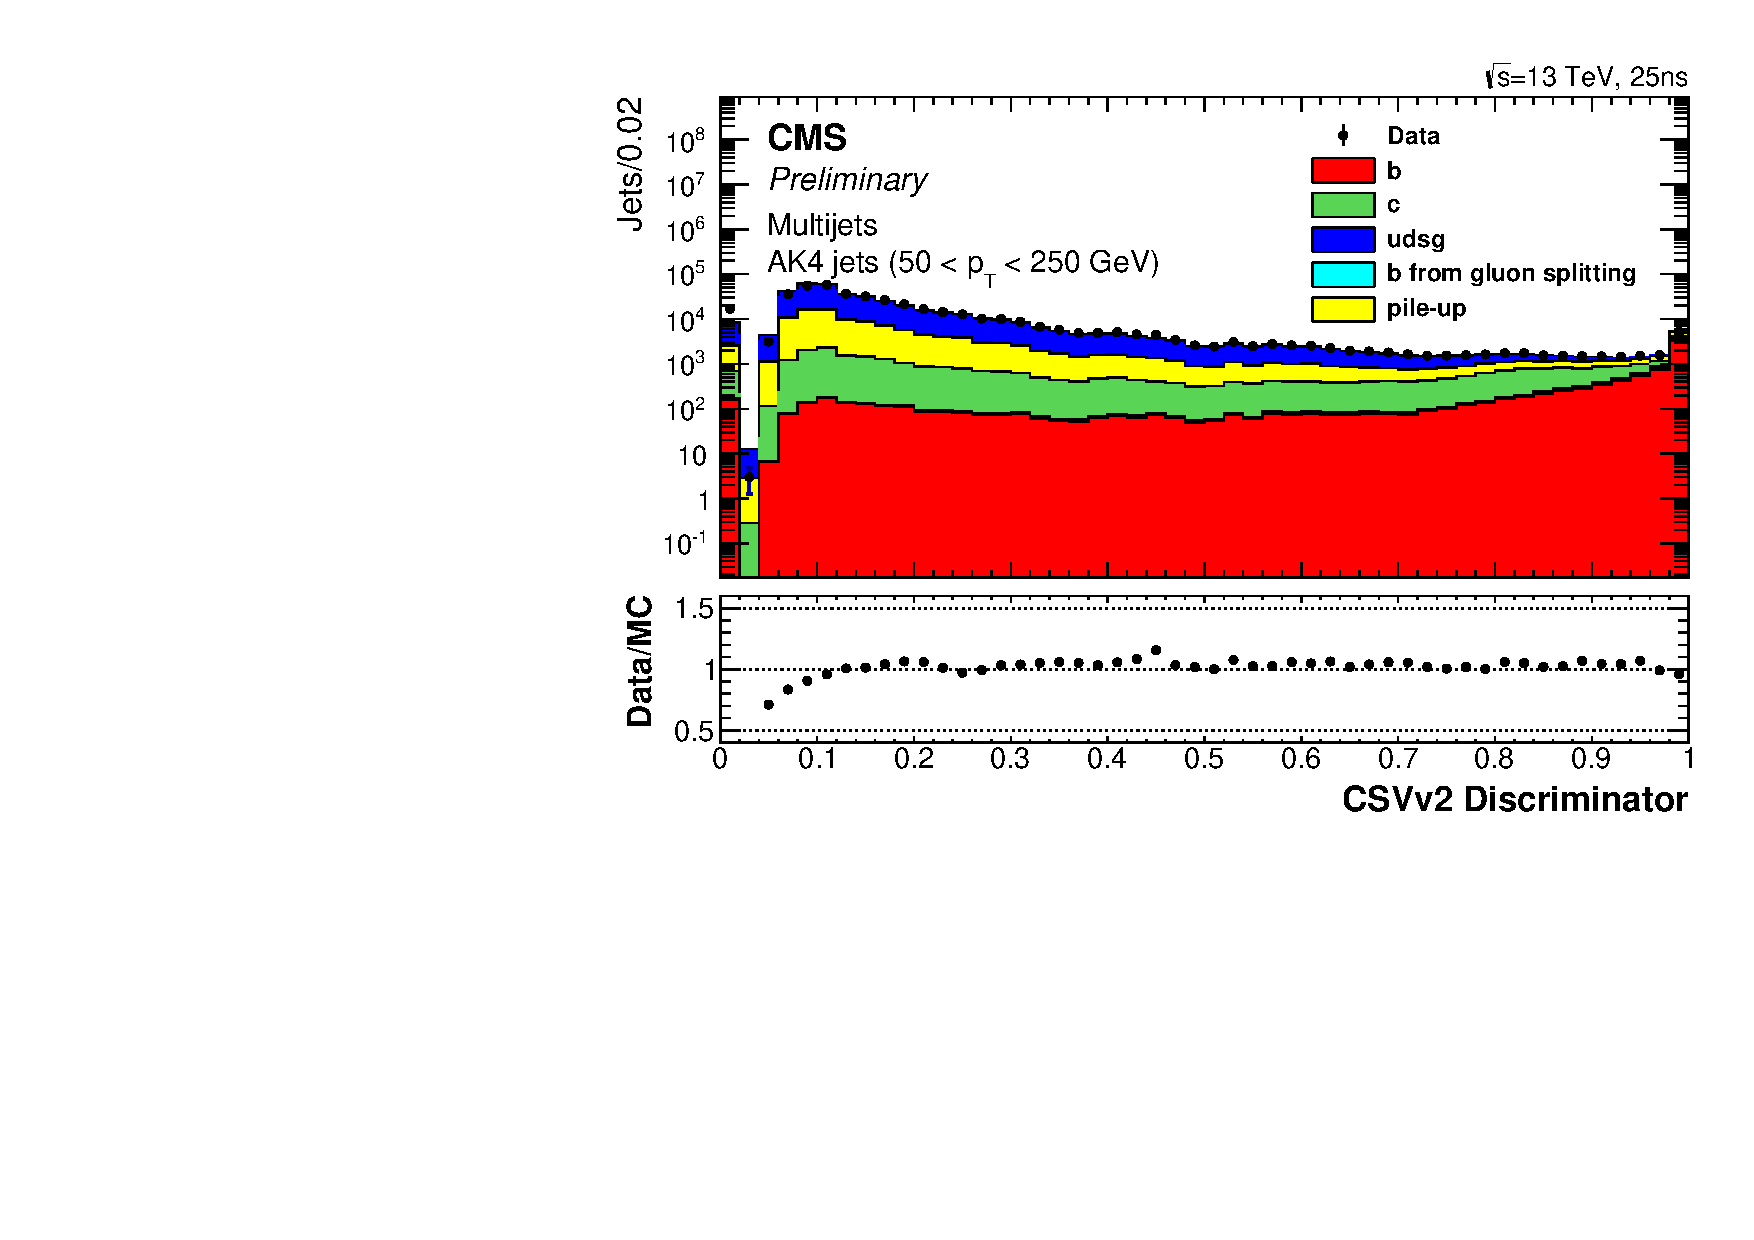
\includegraphics[width=0.5\textwidth]{figs/csvv2_multijet_13TeV.pdf}
\caption{Discriminator values for the CSVv2 algorithm for an inclusive multi-jet topology, where the total number of entries in the simulation is normalized to the observed number of entries in the data.}
\label{fig:CSVv2_multijet}
\end{figure}

%%---------------------- MET definitions ---------------------- %%
\section{Missing transverse energy}
\label{sec:MET}
A crucial aspect of this search requires the precise modeling of the missing transverse momentum, denoted \ptvecmiss, and its magnitude, referred to as the missing transverse energy, and denoted by \ptmiss. Owing to momentum conservation, \ptvecmiss corresponds to the transverse momentum that is carried by weakly interacting particles, such as neutrinos. This observable is of particular importance in the search for \ttDM, since the neutral DM particles are also predicted to interact weakly, hence they will escape the detector volume without being detected. Consequently, the measurement of \ptmiss relies heavily on the detectable and reconstructed physics objects mentioned in the preceding sections. Thus, \ptmiss is defined as the imbalance in the transverse momentum of all particles that interact with the detectors. As mentioned in Sec.~{}, the CMS PF algorithm reconstruction uses all the available detector information to create a list of identified and reconstructed PF particles. It then follows that the \ptvecmiss is defined as the negative vectorial sum of the transverse momenta of all PF particles reconstructed in the event, such that,

\begin{equation}
  \ptvecmiss = -\sum_{i=\mathrm{PF\:particles}}{\vec{\pt}_{i}}
  \label{eq:met}
\end{equation}

The measurement of the \ptmiss can be mismeasured as a cause of a variety of reasons. The nonlinear response of the calorimeter for neutral and charged hadrons due to its noncompensating nature, minimum energy thresholds in the calorimeters, inefficiencies in the tracker, or neutrinos from semileptonic particle decays are a sources from which bias can be introduced in the \ptmiss measurement. In order to mitigate these biases, the \ptmiss derived from PF particles, denoted by PF-\ptmiss, is corrected for using jet energy scale corrections, so Eq.~\ref{eq:met} then becomes,

\begin{equation}
  \mathrm{PF}\ptvecmiss = \mathrm{PF}\ptvecmiss - \sum_{\mathrm{jets}}{\Big(\vec{\pt}^{\mathrm{corr}}_{\mathrm{,jet}} - \vec{\pt}_{\mathrm{,jet}}\Big)}
\end{equation} 

All jets with $\pt > 15\:\GeV$ and less than 0.9 of their energy deposited in the ECAL are corrected. In addition, the muon four-momentum is subtracted from the jet four-momentum when the correction is performed, if a muon is found within a jet. Jet energy corrections consist of several stages and are derived and applied in a factorized manner, although the underlying procedure of scaling the jet four-momentum with a scale factor (SF) which depends on jet quantities such as \pt, \eta, and flavor is universal. The corrections are listed and described briefly below in the order they are applied.

\begin{itemize}
  \item L1 Pile up: Aimed at removing any energy contributions from pile-up events, this correction is determined from a simulation sample of QCD dijet events which are processed with and without pileup overlay. The corrections are parametrized as a function of the jet area (A), jet \eta and \pt, and the offset energy density (\rho). The correction applied to data is parametrized in \eta and determined using zero bias events.
  \item L2L3 MC-truth corrections: The reconstructed jet \pt is compared to the particle level jet \pt in order to derive jet response corrections from a QCD dijet simulation sample. The jet response is made uniform over \pt and \eta, the jet variables in which it is derived.
  \item L2L3 Residuals: These corrections are applied to jets in data and include both an \eta and \pt component. For the \eta dependence (relative corrections), dijet events are compared to a jet of similar \pt in the barrel region ($|\eta|<1.3$). For the \pt dependence (absolute corrections), the JES relative to the reference JES of the barrel jet is taken into account. The jet absolute scale corrections are derived using Z(\mu\mu/$ee$)+jets, photon+jet, and multijet events.
\end{itemize}

%%---------------------- Event selection ---------------------- %%
\section{Event Selection}
\label{sec:selection}

The objects defined in Sec.~\ref{sec:leps}-\ref{sec:MET} are all employed to target the selection of events consistent with \ttMET where both tops have leptonically decaying W bosons. The selection for the signal region is the following,

\begin{itemize}
\item Two ``Tight'' leptons with opposite charge ($ee$ or $e\mu$ or $\mu\mu$) with $\pt>25\:\GeV$ for the leading lepton and $\pt>15\:\GeV$ for the trailing lepton,
\item No additional leptons with $\pt>10\:\GeV$ and passing ``Loose'' muon or ``Veto'' electron criteria,
\item Two or more jets where at least one jet is b-tagged,
\item $M_{\ell\ell}>20\:\GeV$,
\item $|M_{\ell\ell} - M_Z|>15\:\GeV$ for $ee$ and $\mu\mu$ events,
\item $\ptmiss>50\:\GeV$,
\end{itemize}

Dilepton candidate events with an invariant mass $M_{\ell\ell}<20\:\GeV$ are removed in order to suppress any backgrounds from low-mass Drell-Yan processes, as well as any contributions from heavy-flavor resoncances. The requirement for events in the same flavor ($ee$ and $\mu\mu$) channel to have an invariant mass $\pm15\:\GeV$ away from the Z boson pole mass is also used to reject $Z(\ell\ell)$ background events. The moderate requirement of \ptmiss$>50\:\GeV$ aims to further suppress contamination from DY events in the same flavor channel.

\subsection{The \mttll variable}
\label{subsec:mt2ll}
Along with categorization according to lepton flavor (same or opposite), events are also categorized based on the stransverse mass quantity, \mttll, defined as,

\begin{equation}
M_{\text{T2}}^{\ell\ell} = \min_{\vec{p}^{\text{miss}}_{\text{T1}}+\vec{p}^{\text{miss}}_{\text{T2}}=\vec{p}^{\text{miss}}_{\text{T}}}
\left(\max\left[M_{\text{T}}\left(\vec{p}^{\ell_1}_{\text{T}},\vec{p}^{\text{miss}}_{\text{T1}}\right),\:M_{\text{T}}\left(\vec{p}^{\ell_2}_{\text{T}},\vec{p}^{\text{miss}}_{\text{T2}}\right)\right]\right),
\label{eq:mt2ll}
\end{equation}

\mttll is partially motivated from the transverse mass, denoted $M_{\text{T}}\left(\vec{p}^{\ell}_{\text{T}},\vec{p}^{\text{miss}}_{\text{T}}\right)$ in Eq.~\ref{eq:mt2ll}, where the most notable use of \mt is in the measurement of the $W$ boson mass in the $W\rightarrow\ell\nu$ decay mode. The transverse mass, defined in the context of a leptonic $W$ boson decay, is as follows,

\begin{equation}
  M_{\text{T}} = \sqrt{M_{\ell}^{2} + M_{\nu}^{2} + 2(E_{\text{T}}^{\ell}E_{\text{T}}^{\nu} - \vec{p}_{\text{T}}^{\ell}\cdot\vec{p}_{\text{T}}^{\nu})}
\end{equation}

where $M_{\ell}$ and $M_{\nu}$ are the masses of the lepton and neutrino, respectively, and $\vec{p}\
_{\text{T}}^{\ell}$ and $\vec{p}_{\text{T}}^{\nu}$ are their transverse momenta. $E_{\text{T}}^{\ell}$ and $E_{\text{T}}^{\nu}$ denote their transverse energies. 

The utility of $M_{\text{T}}$ is best for cases wherein one missing particle is expected (i.e. the neutrino in the leptonic $W$ decay). However, once more than one missing particle is expected in an event, it is no longer possible to calculate the \mt since the \pt of an individual missing particle cannot be resolved. Recalling that \ttDM production and decay follows this route:

\begin{equation}
pp \rightarrow t\bar{t} + \phi \rightarrow W^{+} b + W^{-} \bar{b} + \chi\bar{\chi} \rightarrow \ell^{+} \nu b + \ell^{-} \bar{\nu} \bar{b} + \chi\bar{\chi},
\end{equation}

a signal event is expected to contain four particles that leave their signature in the detector collectively as \ptmiss, namely the $\nu,\:\bar{\nu},\:\chi,\:\bar{\chi}$. Similarly, in the case of the SM \ttll process, the two lepton neutrinos are the sole contributors to the total \ptvecmiss, and as postulated by the authors in~\cite{Lester:1999tx}, if the $\vec{\pt}^{\nu}$ and $\vec{\pt}^{\bar{\nu}}$ were obtainable, the maximum \mt value is bounded from above by the $W$ boson transverse mass, such that,

\begin{equation}
  M_{W}^{2} \geq \max{\{M_{\text{T}}^{2}\left(\vec{p}^{\ell^{+}}_{\text{T}}, \vec{p}^{\nu}_{\text{T}}\right), M_{\text{T}}^{2}\left(\vec{p}^{\ell^{-}}_{\text{T}}, \vec{p}^{\bar{\nu}}_{\text{T}}\right)\}}
\end{equation} 

The partitioning of the \ptvecmiss is however unknown, so the best that can be assumed is, 

\begin{equation}
  M_{W} \geq M_{\text{T2}}^{\ell\ell} = \min_{\vec{p}^{\text{miss}}_{\text{T1}}+\vec{p}^{\text{miss}}_{\text{T2}}=\vec{p}^{\text{miss}}_{\text{T}}}\left(\max\left\{M_{\text{T}}\left(\vec{p}^{\ell_1}_{\text{T}},\vec{p}^{\text{miss}}_{\text{T1}}\right),\:M_{\text{T}}\left(\vec{p}^{\ell_2}_{\text{T}},\vec{p}^{\text{miss}}_{\text{T2}}\right)\right\}\right).
\label{eq:mt2ll_2}
\end{equation}

The minimization in Eq.~\ref{eq:mt2ll_2} occurs over all the possible two-way partitions of \ptvecmiss in the event. For the case of the SM \ttll background, a kinematic endpoint in the \mttll distribution, shown in~\FigureRef{fig:mt2ll}, occurs at the $W$ boson pole mass. With this in mind, two signal regions are formed using the \mttll variable, where events with \mttll$>110\:\GeV$ comprise the high signal purity region, since the signal is not expected to be contained in the region below the $M_W$ as is the case for the SM \ttll background. The low signal purity category is formed by the remaining events, for which \mttll$<110\:\GeV$.

\begin{figure}
  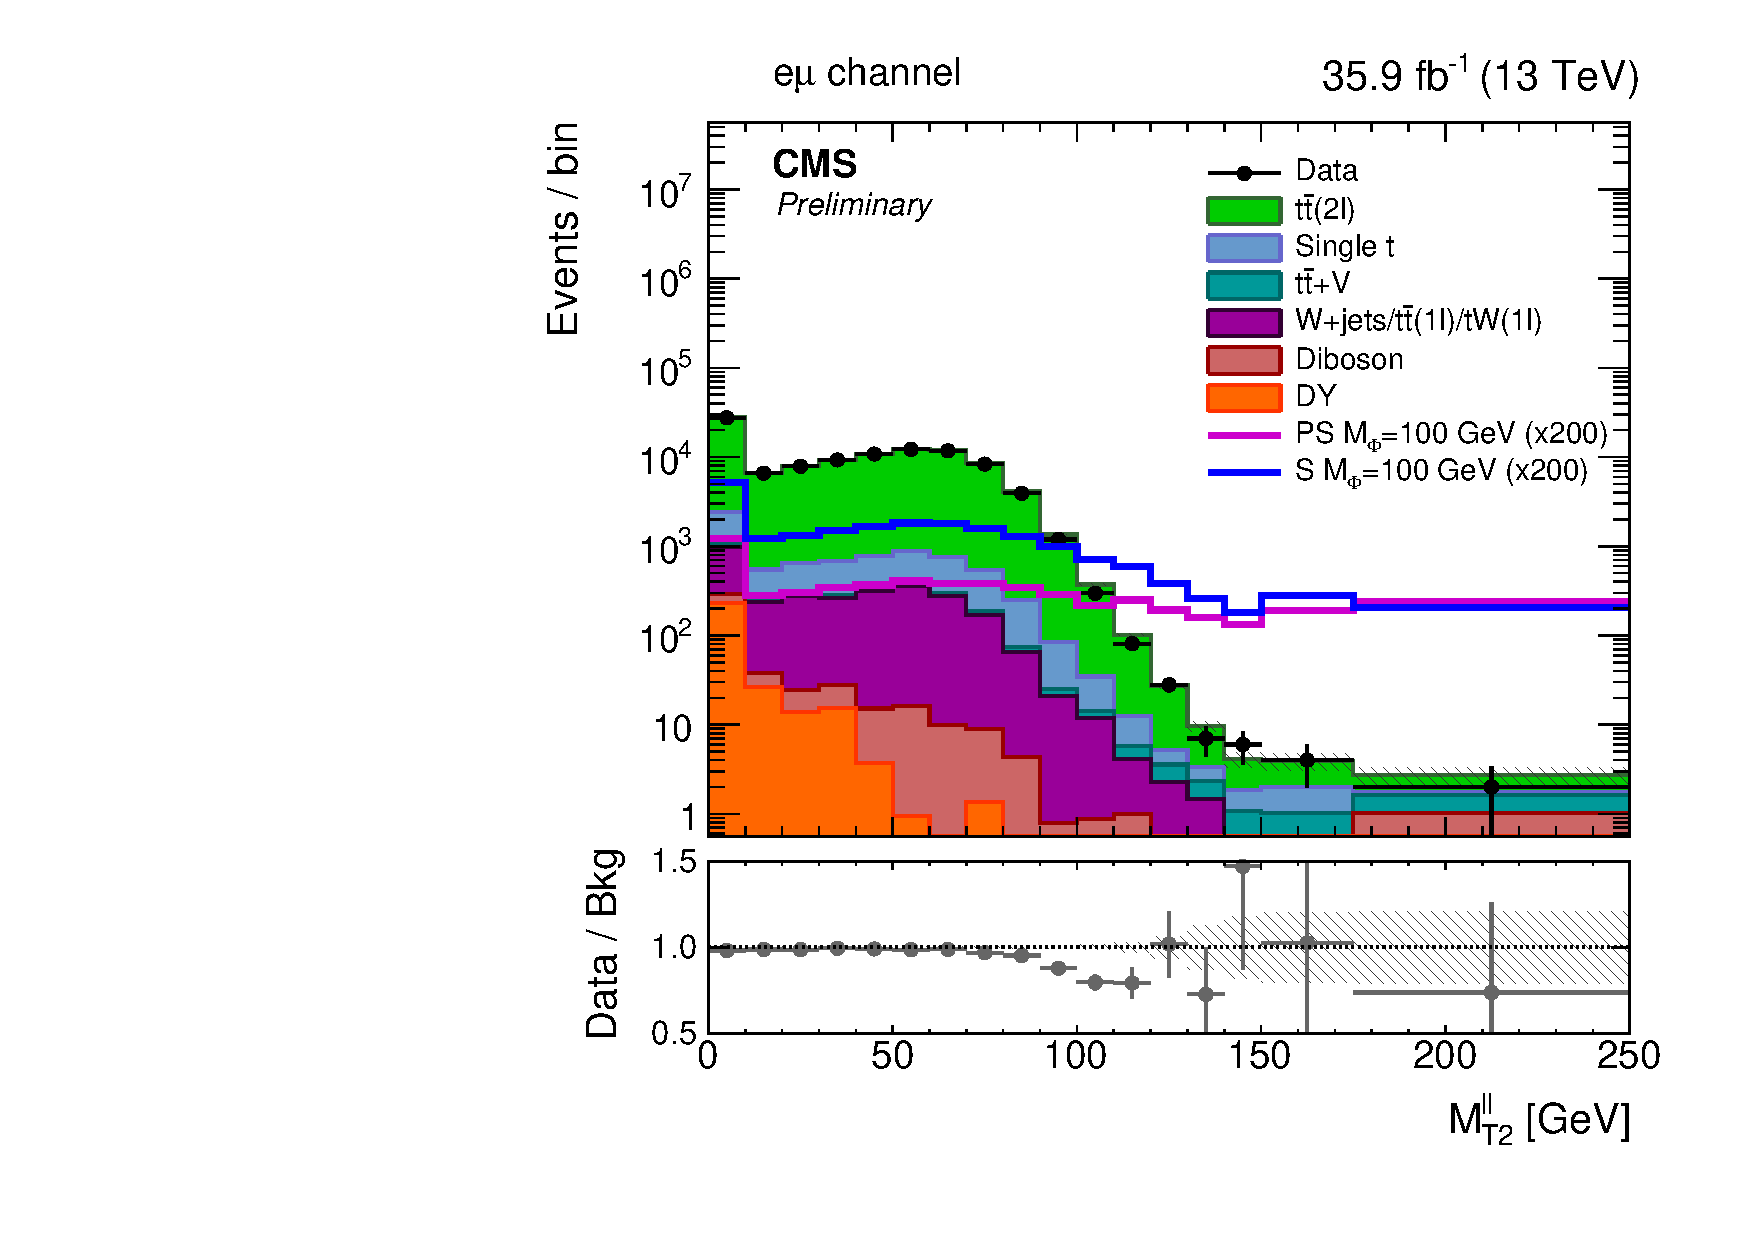
\includegraphics[width=0.6\textwidth]{figs/mt2log_em.pdf}
  \caption{The \mttll distribution in data and simulation for events passing selection requirements for the $e\mu$ channel. The distribution of two example signals (scalar and pseudoscalar mediator, $m_{\phi/a} = 100\:\GeV$) with $m_{\chi}=1\:\GeV$ is scaled up by a factor of 200. The last bin includes overflow. Uncertainties are statistical only.}
  \label{fig:mt2ll}
\end{figure}



\begin{comment}
Here are some funky floats using ``continued captions'', i.e. for a semantically
collected group of float contents which are too numerous to fit into a single
float, such as the pretty circles in the following figure:

\newcommand{\circleimg}[1]{%
\begin{tikzpicture}
  \draw[color=black,fill=#1,thick] (1,0) circle (1.5cm);
\end{tikzpicture}%
}

\begin{figure}[hb]
  \subfloat[][Example 1a]{\label{fig:cc1a}\circleimg{red!80}}\quad
  \subfloat[][Example 1b]{\label{fig:cc1b}\circleimg{green!70!yellow}}\quad
  \subfloat[][Example 1c]{\label{fig:cc1c}\circleimg{blue!80}}\quad
  \subfloat[][Example 1d]{\label{fig:cc1d}\circleimg{orange!80!yellow}}
  \caption{Demonstration of \texttt{subfig} continued captions.}
  \label{fig:cc1}
\end{figure}

\begin{figure}[p]
  \ContinuedFloat
  \subfloat[][Example 1e]{\label{fig:cc1e}\circleimg{violet}}\quad
  \subfloat[][Example 1f]{\label{fig:cc1f}\circleimg{cyan}}\quad
  \subfloat[][Example 1g]{\label{fig:cc1g}\circleimg{magenta}}\quad
  \subfloat[][Example 1h]{\label{fig:cc1h}\circleimg{yellow}}
  \caption[]{Demonstration of \texttt{subfig} continued captions (continued).}
\end{figure}

\noindent
This mechanism means that the same float label is used for both pages of
floats. Note that we can refer to \FigureRef{fig:cc1} in general, or to
\FigureRef{fig:cc1g} on \PageRef{fig:cc1g} in particular!

\noindent
Just for the hell of it, let's also refer to \SectionRef{sec:neutralmixing}.
\end{comment}
